\part{Synthesis}
	\chapter{Introduction}
	Now that the relevant product fields are understood to a sufficient degree and the product's needs have been established we can begin to plan out how we will achieve the project's objectives. First we will established the methological approach that will structure the product's development. Then, for each of the core product requirements we will look at a high level design overview of how the requirement will be met, the actual implementation of this design, and testing to evaluate how well this requirement has been satisfied by this implementation.
	
	\chapter{Methological Approach}
	The project employed a prototyping methodology for development. First, we must perform an investigation into the system requirements, which was performed in the analysis with a list of specific core requirements being outlined in the conclusion. Following this the first prototype is built, which will resemble an incredibly basic scaled down version of how the final system should ideally look. This prototype is then thoroughly evaluated, with potential changes that would bring the prototype closer to the final system being figured out. Finally, these changes are then implemented and the prototype is evaluated once again. This is repeated until the product has reached its ultimate goals.
	
	%prototyping diagram?
	
	This methodology was employed partially due to the hardware nature of the product. Key features of the robot hinged on aspects like movement and observation being possible, so it was important to get a prototype that has this basic functionality up and working and quickly as possible. The prototyping approach allowed a pure focus on getting these functions working, and once they were the robot could be improved iteratively.
	
		\subsection{Initial Prototype}
		As previously stated, this methodology involves an initial prototype that all future prototypes will be an iteration of. The initial prototype of the project will involve the basic, primary construction of the robot. This will first involve the basic chassis assembly followed by attempting to connect relevant components to eachother. Once this is done, we'll hopefully have an incredibly crude robot that won't be capable of anything, but should hopefully serve as a solid foundation for future development toward the project goals.
		
		A similar approach will be followed for processing the map data. It won't be developed simultaneously at first as the robot needs to be capable of storing observational data from the LIDAR before the program can actually do anything, however it will start to be put together once the robot crosses this developmental threshhold.
	
	\chapter{Design}
		\section{Introduction}
		Before implementation of the specific project aims can be implemented, we first need the initial prototype that we can begin iteratively improving. Therefore, it's logical to design the initial robotic prototype first. What follows is an overview of how the initial robot prototype will be designed, followed by a breakdown of each of the individual project aims will be met.
	
		\section{Initial Prototype}
		Here will be the design for the base robot. The aim here is to achieve a solid foundation that all development can build on in order to meet the project objectives.
			\subsection{Hardware}
				\subsubsection{Chassis}
				First off will be the basic assembly of the three wheeled omnidirectional chassis. The chassis is comprised of two triangular metal plates, joined together by metal rods that are screwed into pre drilled holes that line up to eachother. The lower platform is where the motors and mounting points for the omnidirectional wheels are found, so once the plates have been connected the wheels will be pushed onto these mounting points and locked into place. Fig \ref{fig:chassisassembly} shows the assembly document that came with the chassis.
				\begin{figure}[h]
					\centering
					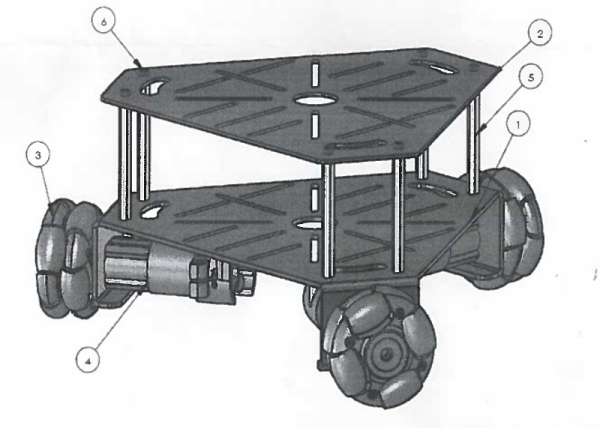
\includegraphics[width=.9\linewidth]{SYNTHESIS/chassisassembly.png}
					\caption{Chassis assembly guide}
					\label{fig:chassisassembly}
				\end{figure}
				
				Now it's time for the microcontroller setup. The microcontroller used in this project is the FRDM-K64F, chosen for it's relatively low cost, small form factor and compatibility with the Micro C Operating System which is being employed for the robot's core program. To control the robot we'll also need a motor driver. The dfRobot Quad Motor Driver Shield is being employed for this project, it can be obtained from Amazon for around \pounds{13}. It was chosen for this relatively low cost, the easily available documentation and the fact that it can easily plug into the FRDM-K64F, the microcontroller of choice for this project. The specifics behind how the shield will be used will be discussed during the movement design section, but in short it allows us to manipulate the energy being sent to the individual wheel motors which will afford us control over how they work and as such control over the robot's movement. Once these two components have been fitted together, the power and ground cables from each of the chassis motors will be plugged into the motor driver shield. Fig \ref{fig:shieldsetup} from the shield's documentation shows an example of this setup with four motors.
				
				\begin{figure}[h]
					\centering
					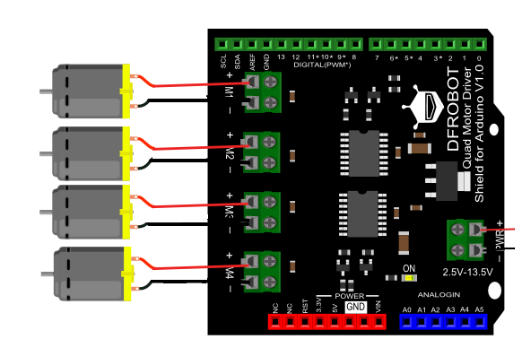
\includegraphics[width=.7\linewidth]{SYNTHESIS/shield_connection.png}
					\caption{Example shield setup}
					\label{fig:shieldsetup}
				\end{figure}
				
				The assembly shouldn't be overly complex, no soldering should be needed to connect components so it should be mostly a case of fitting things together.
				% explain LIDAR later.... :(
				
				\subsubsection{Power}
				The hardware components that will need powering are the three motors used to drive the omnidirectional wheels, the microcontroller, and the LIDAR sensor. Table \ref{table:1} has a run down of these hardware components, the voltages, and the milliamp consumption that they have.
				
				\begin{table}[h]
					\centering
					\begin{tabular}{|| l | l | l ||} 
						\hline
						Component & Voltage & Milliamp \\ [0.5ex] 
						\hline
						3x DC Coreless Motor  & 12V & Up to 1400 mA  \\ 
						FRDM-K64F  & 5 to 9V &  50 mA \\
						RPLIDAR  & 5 to 10V & Up to 1050 mA\\
						\hline
					\end{tabular}
					\caption{Components and respective voltages}
					\label{table:1}
				\end{table}
				
				To save on cost and complexity, it would be ideal to only use a single battery for the robot's power source. A single power source will be used for the robot, a battery holder containing 8 1.5V batteries will give us the 12V we need for the motors. Then, a step down voltage regular will be used to lower the voltage required for the other components. Fig \ref{fig:powersetup} has an overview of this.
				% !!!!!!!!!!!!!!!!!!!!!!!COME BACK TO THIS!!!!!!!!!!!!!!!!
				
				Generally cheaper alkaline batteries have about 1800 to 2800 mAh (milliamp hours) in them, so an 8 pack of these will give us about half an hour's worth of operation before the robot starts to suffer due to low power. This is a worst case scenario assuming a constant high power draw, but this should be sufficient for the purposes of prototyping and demonstration. 
			
			\subsection{Software}
			The software for the actual robot will be written in C++, compiled and deployed onto the microcontroller with the mbed SDK. At its foundation, it will be a Micro C OS with a series of configured tasks to perform various aspects of the robot's functionality. As you would expect, these tasks will come with their own memory tasks and will be designated with appropriate priorities. For the initial setup, we only need to make a skeleton OS to ensure we can properly compile and deploy code onto the microcontroller. Some relevant data structures and variables for task priorities and memory stacks, as well as a single task that prints hello world would be fine for this.
		
		\section{Designing for Requirements}
		Once this incredibly basic initial prototype is in place, we can begin to move toward truly fulfilling the project requirements. What follows is an overview of how each of the different project requirements will be met, with appropriate explanations toward the hardware and software employed.
		
			\subsection{Movement}
			The first of the three product aims outlined in the Analysis is that 'the robot must be capable of movement'.
				\subsubsection{Hardware}
				The previously mentioned dfRobot Quad Motor Driver Shield comes into play here. As shown in fig \ref{fig:shieldsetup}, the motors power and ground cables will connect to the appropriate pins on the shield. The motors can be manipulated once they receive power in this fashion. The shield is able to affect the electricity being sent to the motors by changing its polarity and by using pulse width modularity. By changing the pin to HIGH or LOW, we can affect the direction that the motor spins in (forward or backwards) and pulse width modulation allows us to affect the speed of the motor.
				
				\subsubsection{Software}
				In order to manipulate the motors we'll need some appropriate variables we can use to refer to the pins that the motor power and ground cables are connected to. 
				%talk about pin lineup here and declaration
				% COME BACK TO THIS, TRIGONOMICAL NAVIGATION!

				
			\subsection{Observation}
			The second of the three product aims outlined in the Analysis is that 'the robot must be capable of observation'.
				\subsubsection{Hardware}
				Only one range finder is being used to gather the observation data, the RPLIDAR A1M8 LIDAR sensor. The sensor is composed of a platform with a motor system that spins the range scanner as it takes readings, as well as some pins that can be used for communication. Fig \ref{fig:rplidarconfig} illustrates these components.
				
				\begin{figure}[h]
					\centering
					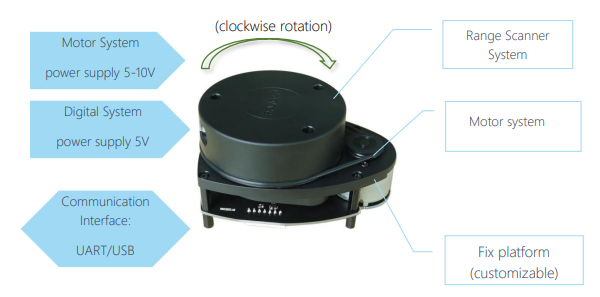
\includegraphics[width=.9\linewidth]{SYNTHESIS/rplidar_configuration.png}
					\caption{Example shield setup}
					\label{fig:rplidarconfig}
				\end{figure}
			
				There are seven pins on the underside of the LIDAR sensor. These pins need to be connected to the appropriate microcontroller ports if the LIDAR is to work. 
				% PICTURE OF LIDAR UNDERSIDE HERE
				
				The GND pins are simple ground pins, they will need to be connected to ground pins on the microcontroller. The RX and TX pins (Recieve and Transmit respectively) are serial pins that will be used for communication with the microcontroller. These LIDAR pins will be linked to their opposite counterparts on the microcontroller (LIDAR RX to Microcontroller TX and vice versa). The V5.0 and VMOTO are simple power pins, they will need to be connected to pins on the microcontroller that output the appropriate amount of voltage. This is how the LIDAR sensor will retrieve power. The MOTOCTL pin is the motor control pin that listens for a signal indicating that a connected device is ready to recieve data. The signal is either high (ready) or low (not ready). To make use of this pin, a generic GPIO pin from the microcontroller will be configured within the microcontroller's software and set to 1 (high) when the robot needs to begin taking scan data.
			
				To interact with the sensor, it will be connected to the robot's microcontroller. We would first need to connect the microcontroller's TX (transmit) and RX (recieve) pins to the LIDAR's inverse pins (TX to RX, RX to TX). Then, using mbed's serial library, we can create a serial variable supplying the microcontroller's connected RX and TX pins and parameters. From this we can invoke methods like putc() and getc(), which put and get characters into and from the serial connection respectively. In order to power the sensor, there are two pins that need to be connected. The first is LIDAR core, which is the power for the actual LIDAR scanner itself. The second is the LIDAR motor, which is what spins the scanner as it makes observations. 
				%COME BACK TO THIS AS WELL...
				
				\subsubsection{Software}
				SLAMTEC have a document detailing the LIDAR protocol. This details the specifics behind how to communicate with the LIDAR. LIDAR communication is primarily achieved through the exchange of data packets. As a basic example, in order to obtain scan measurements the host system first needs to send data packets corresponding to the begin scan command. Once the LIDAR has recieved and processed this, it should begin sending back observational data. 
				
				The format of the requests that need to be sent is documented in the LIDAR's protocol documentation\citep{rplidarprotocol}. To implement this, it would be a good idea to create a data structure in the microcontroller's C++ program with fields listed in the protocol (start flag, command, etc) and then put this field into the serial connection. A similar data structure could be populated with what is recieved from the serial channel to make it easy to process the data.
				
				SLAMTEC provide an SDK for the LIDAR sensor however, which comes in the form of header files which will automatically implement this functionality. Table \ref{table:sdkbreakdown} has a manifest of the SDK and the functionality that it provides.
				
				\begin{table}[h!]
					\centering
					\begin{tabular}{|| l | l ||} 
						\hline
						File & Purpose \\ [0.5ex] 
						\hline
						rplidar.h  & Parent file for subsequent header files  \\ 
						rplidar\textunderscore driver.h  & Provides RPLidarDriver class for  interfacing with sensor   \\
						rplidar\textunderscore  protocol.h  & Defines structs and constants for the LIDAR protocol  \\
						rplidar\textunderscore  cmd.h & Defines request/answer structs for LIDAR protocol  \\ 
						rptypes.h & Platform independent structs and constants  \\ [1ex] 
						\hline
					\end{tabular}
					\caption{RPLIDAR SDK files}
					\label{table:sdkbreakdown}
				\end{table}
				
				Essentially, the C++ program running on the microcontroller would need to create an RPLidarDriver variable which would be used to represent the connected LIDAR sensor. Once this is achieved the premade methods that implement the protocol functionality could be ran to achieve control over the LIDAR.
				
			\subsection{Processing Observational Data}
			The last of the three project objectives is that 'the observational data must be processed into a map'.
				\subsubsection{Hardware}
				Once the robot is receiving data from the LIDAR sensor, it needs to be transferred to an external program where the CSM software can be ran to generate a map from it. To do this a Micro SD-Card will be used. The FRDM-K64F has a Micro SD-Card socket attached to it, and the microcontroller will save the observational data to this card so that after a session of moving and scanning it can be plugged into a machine where it is able to be processed. The University's loans office can provide an 8GB card as well as an adapter allowing it to be plugged into a PC's USB slot, so this approach won't incur any extra cost. The saved data will only be angle and distance measurement pairs, so the card's (relatively) small size won't pose any memory issues. 
				
				\subsubsection{Software}
				First, the microcontroller must save this data to the connected Micro SD-Card. The Mbed microcontroller have a library called SDFileSystem used for interaction with connected SD cards. Using this library, a simple text file will be created on the Micro SD-Card and angle/distance measurements obtained from the LIDAR sensor will be written to it.
				
				Once readings have been written to the SD-Card, it will be removed and plugged into a USB adapter so it can be plugged into a computer. For ease of use, a GUI program will be used to automate the rest of the functionality. To design the GUI, a Python library called Tkinter will be used. It offers all the widgets that will need to be used to make a basic GUI such as frames, buttons and labels and its support of most (if not all) operating systems will allow it to be easily used. The GUI's job then is to create an appropriate input for CSM and to use it to generate a map from the readings. CSM takes in readings in the form of either a json or a carmen log. Of the two, json will be used due to its familiarity and much more easily accessible documentation around the internet. To invoke the CSM software itself via the program, Python features a subprocess module which allows for Python programs to spawn simple subprocesses and retrieve information they return. Once the software has processed a map from the readings, it will be output onto the screen so that the user can view it.
		
		\section{Pseudo Code}
		Some pseudo code follows to help represent the initial plan for the code's structure and functional breakdown.
		%PSEUDO CODE HERE, COPY FINAL ROBOT CODE
		
	\chapter{Implementation}
		\section{Introduction}
		\section{Initial Prototype}
			\subsection{Hardware}
			\subsection{Software}
		\section{Implementing Requirements}
			\subsection{Movement}
				\subsubsection{Hardware}
				\subsubsection{Software}
			\subsection{Observation}
			Implementation of the robot's ability to take observations about its environment first involved a hardware configuration. The LIDAR sensor needed to be connected to the microcontroller so that it could draw power from the battery, as well as communicate with the microcontroller allowing it to receive commands and send observational data. Once the hardware connection was established, software on the microcontroller had to be capable of operating the LIDAR sensor and recieving its observations.
				\subsubsection{Hardware}
				As previously discussed, the seven pins on the underside of the LIDAR sensor need to be correctly connected up to the appropriate microcontroller pins if the sensor is to be used.
				
				Table \ref{table:4} gives an overview of which LIDAR pins needed to be connected to which microcontroller pins.
				
				\begin{table}[h!]
					\centering
					\begin{tabular}{|| l | l | l ||} 
						\hline
						LIDAR Pin & K64F Pin & Pin Purpose \\ [0.5ex] 
						\hline
						GND  & GND & Ground  \\ 
						RX  & TX  & Serial Communication \\
						TX  & RX & Serial Communication \\
						V5.0 & 5v & LIDAR Core Power \\ 
						GND & GND & Ground \\ 
						MOTOCTL & D7 & DTR (Data Terminal Ready) \\ 
						VMOTO & 3v3 & LIDAR Motor Power \\ [1ex] 
						\hline
					\end{tabular}
					\caption{RPLIDAR SDK files}
					\label{table:3}
				\end{table}
			
				Due to the dfRobot Quad Motor shield being plugged into the K64F microcontroller, these LIDAR pins need to be connected to ports on the robot shield that are plugged into the appropriate microcontroller pins. Essentially, we look at what port needs to be used on the underlying microcontroller, then plug it into the motor shield port that is sitting on top of it. The LIDAR pins and shield ports were connected using simple male to female connector wires.
				
				Once this was done, the LIDAR was able to function mechanically.
				
				\subsubsection{Software}
				Following the hardware setup the microcontroller needs to actually communicate with the LIDAR sensor so that it can send commands, as well as receive observational data. 
				
				To first of all ensure the LIDAR is ready to communicate, the previously discussed MOTOCTL pin on the LIDAR needs to be recieving a HIGH signal so that it knows the microcontroller is ready to begin recieving data. The K64F features numerous GPIO pins that can be easily configured for usage in situations like this. One such pin (D7) was simply declared as a basic DigitalOut allowing the microcontroller to manipulate the pin's polarity.
				
				% too granular?
				\begin{lstlisting}
				DigitalOut dtr(D7);
				\end{lstlisting}
				
				When we want the sensor to output data this pin can be set to HIGH...
				\begin{lstlisting}
				dtr = 1;
				\end{lstlisting}
				
				...or when we want it to stop, we can set it to LOW.
				\begin{lstlisting}
				dtr = 0;
				\end{lstlisting}
				
				Once this was done and the DTR pin was set to HIGH, the LIDAR began spinning. The microcontroller didn't instantly begin recieving data however, as simply connecting the LIDAR and microcontroller serial pins are not enough for communication. In order to interact with the serial channel it needs to be declared in the robot's core program as an appropriate variable. There exists a library for arm MBED microcontroller called BufferedSerial which can be used for this. The original Serial library that it is based on allows for serial communication, with BufferedSerial simply adding a buffer to this. The core functionality remains the same however.
				
				First the pins being used for serial communication need to be declared as a BufferedSerial variable, with BufferedSerial taking the TX and RX pin (in that order) of the microcontroller. 
				\begin{lstlisting}
				BufferedSerial lidar_device(D1, D0);
				\end{lstlisting}
				
				As previously discussed in the Design, SLAMTEC has an SDK that automates most of the LIDAR functionality. The appropriate files were added to the project and made able to be used by the core program with a simple include statement at the top of the main.cpp file.
				\begin{lstlisting}
				RPLidar lidar;
				\end{lstlisting}
				
				Following this a base lidar variable can be declared from the RPLidar class the SDK adds.
				\begin{lstlisting}
				RPLidar lidar;
				\end{lstlisting}
				
				Once this variable has been declared, in the program's main method the DTR is set to 0 to ensure that the LIDAR won't start scanning and outputting data when we don't need it to. The LIDAR variable is then connected to the relevant serial variable (the previously declared BufferedSerial) and the start scan command is issued. Despite receiving the command to start scanning the LIDAR won't begin until the DTR gives it the go ahead, but by configuring this as soon as the program begins it's a lot easier to stop and start the LIDAR data output.
				\begin{lstlisting}
				dtr = 0;
				lidar.begin(lidar_device);
				lidar.startScan();
				\end{lstlisting}
				
				From here, two different simple one-line methods are used to start and stop the lidar.
				\begin{lstlisting}
				static void beginScanning() {
					dtr = 1;
				}
				
				static void stopScanning() {
					dtr = 0;
				}
				\end{lstlisting}
				These methods allow for quick and easy configuring of the DTR pin.
				
				Now that the LIDAR is configured and can begin sending out data, it's time to start actually storing it within the program. First we need appropriate mediums for the storage of LIDAR data. This entails something to store a LIDAR sample that has just arrived so we can manipulate it to take what we need from it, and also a buffer to store all the total readings collect so that they can later be written to disk. 
				
				In order to store a newly recieving reading, the RPLidar SDK implements a basic struct that can be filled in with a .getCurrentPoint() method. This will be used so that recieved readings can be easily manipulated.
				\begin{lstlisting}
				struct RPLidarMeasurement
				{
					float distance;
					float angle;
					uint8_t quality;
					bool  startBit;
				};
				\end{lstlisting}
				
				Now we need somewhere to store the readings themselves so they can be written to disk later on. We're interested in storing a large number of angle/distance pairs, so a large two dimensional array was used.
				\begin{lstlisting}
				float readingsBuffer[16000][2];
				\end{lstlisting}
				A two dimensional array was used to ensure an understandable format to the array. The array has 16000 spaces, with each space storing two seperate float values (angle and distance respectively). Now the actual method to take LIDAR readings and store them in the buffer needs to be made.
				
				Now that readings can be manipulated and stored, it's time to properly implement the method that stores them to a buffer.
				\begin{lstlisting}
				static void takeReadings() {
					int arraySize = (sizeof(readingsBuffer)/sizeof(float))/2;
					struct RPLidarMeasurement measurement;
					for(int i = 0; i < arraySize; i++) {
						lidar.waitPoint();
						measurement = lidar.getCurrentPoint();
						readingsBuffer[i][0] = measurement.angle;
						readingsBuffer[i][1] = measurement.distance;
					}
				}
				\end{lstlisting}
				The method iterates through the buffer and stores the angle and distance of each reading it receives.
				
				All of these methods can now be incorporated into the scan task.
				\begin{lstlisting}
				static void appTaskScan(void *pdata) {
					uint8_t status;
				
					while(true) {
						OSSemPend(readyToScan, 0, &status);
						pc.printf("Scanning...\n");
						beginScanning();
						takeReadings();
						stopScanning();
						pc.printf("Stopping scan.\n");
						status = OSSemPost(readyToScan);
						OSTimeDlyHMSM(0,0,0,4);
					}
				}
				\end{lstlisting}
				Once the readyToScan semaphore has been released, the LIDAR begins scanning, stores the readings to the buffer and then stops scanning. It then released the semaphore so that the robot can go back to moving.				
				
			\subsection{Processing Observational Data}
				\subsubsection{Hardware}
				\subsubsection{Software}
	
	
	\chapter{Testing}
		\section{Introduction}
		\section{Initial Prototype}
			\subsection{Hardware}
			\subsection{Software}
		\section{Implementing Requirements}
			\subsection{Movement}
				\subsubsection{Hardware}
				\subsubsection{Software}
			\subsection{Observation}
				\subsubsection{Hardware}
				\subsubsection{Software}
			\subsection{Processing Observational Data}
				\subsubsection{Hardware}
				\subsubsection{Software}
				
	\chapter{Previous Failed Attempts}
		\section{Observation}
	